\section{Dealing with diachronic files}
The Meso-NH program of post-processing ({\sc diag}) treats synchronous 
files from initialization or simulation. 
For a given need, one wants to work on fields stored in
a diachronic file before exploration with {\tt diaprog} or with another
graphical tool to possibly compare with observations.

\begin{itemize}
\item The \texttt{extractdia} tool allows to extract fields from a diachronic 
file, on the whole domain or on a part of it, to interpole them (horizontal
grid and/or vertical grid) and to write 
them in some other given formats (section \ref{extractdia}). 
This program is based on a routine of reading and a routine of writing of 
diachronic variables: 
they are the essential source lines to deal with a diachronic file.
These 2 routines can be used in the user own program to match his personal
needs. An example of such a program \texttt{exrwdia.f90} and how to compile it
is given in section \ref{exrwdia}.
\end{itemize}

Some other tools based on the 2 routines of reading and writing
are also available to allow easier comparisons with observation 
data (sections \ref{mnh2obs} and \ref{obs2mnh}):
\begin{itemize}
\item \texttt{mesonh2obs} to get MesoNH field values at given 
observation points (the format of output file is ASCII),
\item \texttt{obs2mesonh} to put observation values on a
given MesoNH grid (the output file has diachronic FM format),
observations can then be plotted with \texttt{diaprog} tool.
\item \texttt{compute\_r00\_pc} to catenate evolution of Lagrangian tracers 
back to the model start (as done in {\sc diag} program, see documentation 
``Lagrangian trajectory and air-mass tracking analyses with
MesoNH by means of Eulerian passive tracers'', Gheusi and Stein, 2005).
\end{itemize}

The figure \ref{outils_dia} resumes the input and output of these tools.
\begin{figure}[htb] 
\centerline{\psfig{file=outils_dia.eps,width=10cm,angle=270} } 
\caption{\label{outils_dia}}
\end{figure}
\\

\underline{Remark}:
 for all the following tools, the input diachronic files can be located
in another directory than the one in which the tool is invoked (as
for \texttt{diaprog}). In this case, initialise the following shell variable
\begin{verbatim}
export DIRLFI=directory_files_diachro
\end{verbatim}

Shell links will be automatically performed during the execution and
will be removed by the mesonh-shell-tool \texttt{rmlink} at the execution end.


\subsection{Extracte fields, domain, change format with
{\tt extractdia} tool}\label{extractdia}

The input file is a FM diachronic file, either a `true' diachronic one 
(its name is ended by {\bf .000} and it contains time series of informations 
obtained during the run of the model),
or a `pseudo'-diachronic one (it is the result of the conversion of a 
synchronous file, see section \ref{diachro_file}), compressed (with {\tt lfiz})
or not.

The format of the output file is chosen by the user among one of the following:
\begin{itemize}
\item a FM {\sc diac}hronic file, 
\item an ASCII file with 
{\sc l}atitude-{\sc l}ongitude-{\sc h}eight-{\sc v}alue or
latitude-longitude-height-value,
\item ASCII files with {\sc free} format defined by the user (one file per field),
\item a {\sc cdl} file (converted to NetCDF format at the end of the program,
with \texttt{ncgen} utility of NetCDF package inside the mesonh-shell-tool \texttt{tonetcdf}),
\item a {\sc grib} file (in the future),
\item a {\sc Vis5D} file (in the future).
\end{itemize}
The main program is an interactive one: 
the name of input diachronic file, the output format, 
the coordinates of the part of the domain,
the name of fields to be read and written are required.
All that is typed on keyboard is saved in {\tt dirextr.}fmt
file, it can be appended and used as input (after renaming it) for the next call
of the tool \\
(e.g. {\tt mv dirextr.DIAC dirDIAC1 ; extractdia < dirDIAC1}).
\\
\\
The advantages for each output format are the following:

\begin{itemize}
\item the wind direction (dd) and wind intensity (ff) could be asked.
\item fields are eventually interpolated according output format,
first vertically and then horizontally.
For vertical interpolation, the user specifies the type of levels (Z or P), 
the number of levels and their values (in m or in hPa). No vertical interpolation if the type of levels is K (model levels).

For horizontal interpolation on regular grid in longitude and latitude, the program chooses the optimum values computed for the model grid. 

If interpolations are required, the wind components are transformed in zonal and meridian components.

These interpolations do not allow interpolation in a required cross-section, the {\sc ficval} file obtained during a {\tt diaprog} session gives this interpolation.
\item for the {\sc diac}hronic format, the output file will be reduced in size
since it contains only some fields on a part of the domain without any interpolations .
It can still be plotted with {\tt diaprog}.
\item for the {\sc ll*v}/ll*v format, the fields can be interpolated onto a 
regular grid in longitude and latitude ({\sc lalo} option) or can remained on 
the conformal model grid.
({\sc llzv}/llzv option for interpolation on constant altitude levels,
{\sc llpv}/llpv option for interpolation on constant pression levels
{\sc llhv}/lhzv option to stay on MesoNH vertical levels).
Three header lines give zoom, unit, variable name and temporal informations and
are followed by four values on each line.
\item for the {\sc cdl} format, the fields can be horizontally interpolated
onto a regular grid in longitude and latitude ({\sc lalo} option),
and eventually vertically on some prescribed levels 
({\sc zcdl} option for interpolation on constant altitude levels,
{\sc pcdl} option for interpolation on constant pression levels,
{\sc kcdl} option to stay on MesoNH vertical levels).
The CDL format is transformed to binary Netdcf format at the end of the program run by the mesonh-shell-tool \texttt{tonetcdf}.
\item the {\sc free} format allows to get the interpolated values (vertical or horizontal interpolations) without any geographical locations: just values list are available after one header line.
\ignore{
\item for the {\sc grib} format, the fields can be horizontally interpolated
onto a regular grid in longitude and latitude and are vertically interpolated
on constant Z-levels or P-levels.
}%ignore
\end{itemize}


\subsection{Personal modifications: \texttt{exrwdia} program}\label{exrwdia}
The \texttt{extractdia} program uses 2 routines of reading
(\texttt{readvar.f90}) and writing (\texttt{writevar.f90}) of MesoNH variables
as they are stored in diachronic files (that is in 6-dimensional arrays).
These 2 routines can be used in your own program:
an example of such a program is \texttt{exrwdia.f90}.
The source code contains extended comments,
and there are some examples of computation with the extracted fields 
(module and direction of components of wind, interpolation on some Z levels, 
maximum of a 3D field along the vertical direction, vertical average between two
Z levels). 

The use of this method need to be familiar with the Mesonh specificities:
 seven grids (Gal-Chen) for the storage of the variables, the U,V wind components are
 referenced in the Mesonh grid and are different from the Uzonal and Vmeridian
 components.

\subsubsection{Routines of reading and writing}
A diachronic file contain time series of informations that are
self-documented (section \ref{diachro_file}). 
The self-documentation is provided by the header of the file, which contains
a list of pre-defined records, and each field (or information)
is stored by several records, the number of them varies
from 8 to 11, according to the type of the information
({\sc cart, mask, spxy, ssol, drst, rspl} or {\sc rapl}).

The subroutine \texttt{readvar.f90} reads the required field. At the first call,
the file is opened, its header is read 
(the dimensions of the total domain ({\sc imax, jmax, kmax}), 
the orography...)
and some characteristics are computed
(the conformal coordinates, the map factor...).
The required field is then read and available in a 6-dimensional array: 
{\sc xvar}(i,j,k,t,n,p)\footnote{For a whole description of the diachronic file
type, reader must refer to the original documentation on the Meso-NH web site:
``{\sc cr\'eation et exploitation de fichiers diachroniques}, J. Duron''.}.

The subroutine \texttt{writevar.f90} writes the field if the wanted output
format is {\sc dia}chronic one.
If it is the first call the header is written, then
the field is stored by the same number of records than when it was read.


The personal code can be inserted in the main program between the call of the
two previous subroutines. For the {\sc free} format, the writing code lines
are to be written in the main program.

\subsubsection{Compilation}
You have to 
\begin{itemize}
\item create a sub-directory {\tt src} to put your own source files
\item copy {\tt\$MESONH/MAKE/tools/diachro/src/EXTRACTDIA/exrwdia.f90} to {\tt src/my\_prog.f90} and modify it
\item initialize the shell variable {\tt ARCH} which refers to your system and the compiler used (see 
examples as the suffix of files in {\tt \$MESONH/MAKE/conf} directory).
\item compile with \\
{\tt gmaketools PROG=my\_prog OBJS="my\_routine1.o my\_routine2.o" } \\ 
(the \$MESONH/MAKE/tools/diachro/{\tt Makefile.exrwdia} version will be used).
\end{itemize}

\noindent To update the routines dependances directly inside the  Makefile:
\begin{itemize}
\item initialize the following shell variables:
\begin{itemize}
\item {\tt MNH\_LIBTOOLS} which is the directory where the reference sources
for the libraries and tools are,
\item {\tt ARCH} which refers to your system and the compiler used (see 
examples as the suffix of files in {\tt \$MNH\_LIBTOOLS/conf} directory). 
\end{itemize}
\item copy the {\tt \$MNH\_LIBTOOLS/tools/diachro/Makefile.exrwdia} file in your working directory, 
rename it to \texttt{Makefile},
\item compile with {\tt gmake}
\end{itemize}


\subsection{Compare to observations with 
{\tt mesonh2obs} tool \label{mnh2obs}}
\subsubsection{Input and output}
The \texttt{mesonh2obs} tool allows to interpolate MesoNH fields 
at given points (such as points where observation data are available). 

The input files are an ASCII file indicated the position of the points by their
latitude and longitude coordinates as well as vertical dimension if a vertical profile is required, and one or several diachronic FM file(s) with fields to interpolate
at previous points.

Each output file, one for each input FM file, is an ASCII one with six possible
options for lines format
(\textsc{llhv}, llhv, \textsc{llzv}, llzv, \textsc{llpv}, llpv).

In the input ASCII file, each line indicates the location of one point,
all lines have the same format, one of the following :\\
\begin{tabular}{l|ll}
 lon lat & and altitudes will be asked by the {\tt mesonh2obs} program\\
 lat lon & and altitudes will be asked by the {\tt mesonh2obs} program\\
 lon lat altitude(m) & \\
 lat lon altitude(m) & \\   
\end{tabular} \\

The output ASCII file contains lines with the same format, one of the 
following according to the option: \\
\begin{tabular}{l|ll}
 lon lat model\_level\_altitude(m)& option \textsc{llhv} \\
 lat lon model\_level\_altitude(m)& option llhv \\
 lon lat altitude(m) & option \textsc{llzv}&
 --interpolation routine \texttt{zinter.f90} for 3D fields\\
 lat lon altitude(m) & option llzv& \hspace*{1cm} " \\
 lon lat pression(hPa) & option \textsc{llpv} &
 --interpolation routine \texttt{pinter.f90} for 3D fields\\
 lat lon pression(hPa) & option llpv& \hspace*{1cm} "   (pressure variable is read in input FM file) \\
\end{tabular} \\


\subsubsection{Usage}
The tool is an interactive one: the option for the lines format of the output
file, the name of the ASCII file with the location of
the observation points are first asked. 
Then the name of the input diachronic files is asked in a loop, and the 
name of the fields to interpolate in a second loop:
\begin{verbatim}
    mesonh2obs << eof
format_output_file # line format of output file (LLHV/llhv/LLZV/llzv/LLPV/llpv)
format_input_file  # LL (lon,lat)ou ll (lat,lon)
altitude_in_input_file # O (altitude_in_m on the third colon)/N 
if N, number_vertical_levels # number of vertical levels above 
                             # each lat,lon points
      list_of_these_levels   # exemple: (in metres or hPa): 500 1500
obs_file                   # name of the Obs file 
0                          # control prints (0/1/2/3)
diachronic_file1           # file with fields to be interpolated (without .lfi)
field1_of_diachronic_file1 # field to be interpolated
field2_of_diachronic_file1
END                        # end of extraction in diachronic_file1
diachronic_file2           # file with fields to be interpolated (without .lfi)
fieldi_of_diachronic_file2 # field to be interpolated
fieldj_of_diachronic_file2
END                        # end of extraction in diachronic_file2
END                        # end of diachronic files list
eof
\end{verbatim}
 
 If \texttt{field\_of\_diachronic\_file} contains 'AC' string 
(for ACcumulated precipitation), you can substract values of the same field
from a previous diachronic file. Then after line 
\texttt{field('AC')\_of\_diachronic\_file}, answer the question: 
\begin{verbatim}
"- ACcumulated rain, do you want to make difference with a previous instant
(o\/O\/y\/Y\/n\/N) ?"
\end{verbatim}
if \texttt{Y$/$O}, indicate the name of \texttt{diachronic\_file\_previous}
(without .lfi) in a second supplementary line. 

\subsubsection{Method}
The main program retrieves first the $X$ and $Y$ conformal coordinates of each 
observation point, then for each read field interpolates it vertically 
if required (vertical profile field with option \textsc{llzv}, llzv, \textsc{llpv} or llpv, \textsc{llhv}, llhv),
and finally interpolates horizontally the field and the array of the vertical
profile.




\subsection{Compare to observations with 
\texttt{obs2mesonh} tool \label{obs2mnh}}
\subsubsection{Input and output}
The \texttt{obs2mesonh} tool allows to replace observations on a MesoNH grid.
The output file has diachronic FM format: it can be used as input for 
\texttt{diaprog} to plot observations in the same background as MesoNH fields.

The input files are one or several ASCII file(s), each of it contains the
values of one type of observation (one value per line, all lines have the same
format: (date-)lon-lat-(alt\_in\_meters-)value or 
(date-)lat-lon-(alt\_in\_meters-)value),
and a diachronic FM file which spatial grid will be
used to replace previous observation values.

The output file is a diachronic file with the orography and the grids of the
input diachronic one, each field corresponds to each input observation file.
One or two fields are added for each observation field treated: N\_field\_name 
for the number of observation averaged in each grid points and if 2D type, ALT\_field\_name for the altitudes of the observation.

\subsubsection{Usage}
The tool is an interactive one:
\begin{verbatim}
    obs2mesonh << eof
file_diachronic_with_zs    # initialize MesoNH spatial and temporal grids
0/1/2/3                 # verbosity level
LL                      # format of obs file (LL=lon lat alt value, 
                        #                     ll=lat lon alt value)
file1_obs               # name of obs file (undefined value=999.0)
name_new_field1         # name of the obs field  in output file
unit_new_field1         # free characters string for unit
1D/2D/3D                # profil of the  obs field 
                        # for the 2D case, only K=1 will be initialised
LL                      # format of obs file (LL=lon lat alt value, 
                        #                     ll=lat lon alt value)
file2_obs
name_new_field2
unit_new_field2
1D/2D/3D
END                     # closing of output diachronic file
eof
\end{verbatim}

\subsubsection{Method}
For each observation read in an input file: \\
- the MesoNH grid point I,J containing this observation is searching, \\
- then for observation with 3D profil, the vertical level K is searched
(the MesoNH vertical grid (Gal-Chen) at I,J is taken into account); 
for observation with 2D or 1D profil, the first level K=1 is attributed,\\
- the value of the observation is stored on grid point (I,J,K). \\
If several values are stored at the same grid point, arithmetic average of 
values is done (when unit is $dBz$, the average is computed in $Ze$).
If there is no values at a grid point, undefined value is put. 
The observations whose altitude is below the altitude of the first MesoNH level are stored at level K=1, a warning message is printed in this case.

The wind components are considered zonal and meridian in the observation and
are transformed to wind components in the Mesonh grid.

\subsubsection{Plotting with \texttt{diaprog}}
For plotting observation values with \texttt{diaprog}, you have to use the
pixel mode
\texttt{LSPOT=T}: this option is recommended for sparse data since there is
no interpolation of values for graphic plotting.
For superpose with simulated field, do not forget to fix the extrema
and interval of plotting for the 2 fields in order to compare them.
Here is an example of directives for \texttt{diaprog} to plot observed values
and superpose them with simulated fields:
\begin{verbatim}
LINVWB=T
!
LCOLAREA=T LISO=F 
LSPOT=T    ! no interpolation 
_file1_'file_obs'
T2M
y          ! yes to draw a black line around obs pixel
0 0
!
_file2_'file_sim'
NIMNMX=1 XDIAINT_T2M=2. XISOMIN_T2M=-8. XISOMAX_T2M=24.
T2M_ON_    ! for superpose
n          ! no black border
T2M_file1_
y          ! yes to draw a black line around obs pixel
0 0
quit
\end{verbatim}


\subsection{Catenation of Lagrangian trajectory with
\texttt{compute\_r00\_pc} tool}
\subsubsection{Input and output}
The \texttt{compute\_r00\_pc} tool allows to compute advanced 
diagnostics. 
related to Lagrangian tracers activated during the model simulation
(\texttt{LLG=.TRUE.} in namelist \texttt{NAM\_CONF}): it is based on the subroutine \texttt{compute\_r00} used in the DIAG program.
See section 2.2 of documentation
``Lagrangian trajectory and air-mass tracking analyses with
MesoNH by means of Eulerian passive tracers'' (Gheusi and Stein, 2005).

The input files are one or several diachronic FM file(s) containing Lagrangian
tracers (\texttt{LGXM,LGYM,LGZM}) simply converted by \texttt{conv2dia} after
simulation, or after {\sc diag} (in the latter case, only Lagrangian
basic diagnostics were asked: \texttt{LTRAJ=.TRUE.} 
in namelist \texttt{NAM\_DIAG} with the namelist
\texttt{NAM\_STO\_FILE} empty, and additional diagnostic fields can be asked:
\texttt{CISO='EV'} and \texttt{LMOIST\_E=.T.} 
for the example of \ref{sss:compute.nam}), 
and an ASCII file named \texttt{compute\_r00.nam} with namelist format.

The output file is a diachronic file containing advanced diagnostics: initial
 coordinates resulting from catenation process, initial values of basic 
diagnostic fields (present in the input diachronic files) that the Lagrangian
parcels had at initial time(s). 


\subsubsection{Usage} \label{sss:compute.nam}
The ASCII file \texttt{compute\_r00.nam} looks as the following:
\begin{verbatim}
&NAM_STO_FILE CFILES(1)='AR40_mc2_19990921.00d.Z',
              CFILES(2)='AR40_mc2_19990920.12d.Z',
              CFILES(3)='AR40_mc2_19990920.00d.Z',
              CFILES(4)='AR40_mc2_19990919.12d.Z', 
              CFILES(5)='AR40_mc2_19990919.00d.Z',
              NSTART_SUPP(1)=3                   /
&NAM_FIELD  CFIELD_LAG(1)='THETAE',
            CFIELD_LAG(2)='POVOM' /
\end{verbatim}
The namelist \texttt{NAM\_STO\_FILE} is the same as in the file
 \texttt{DIAG1.nam}. The namelist \texttt{NAM\_FIELD} indicates the other
quantities for which initial values have to be computed.
\\

Then to run the tool,
\begin{verbatim}
#  initialise the following shell variable (optional if input file 
#  is in the current directory):
export DIRLFI=directory_files_diachro
#  initialise the variable ARCH (LXNAGf95 for PC, HPf90 for HP)
export ARCH=LXNAGf95
#  execute 
$MESONH/MAKE/tools/diachro/$ARCH/compute_r00_pc
\end{verbatim}



\subsubsection{Method}
The structure of the program and the interpolation subroutine
 (\texttt{interpxyz}) are the same as in the {\sc diag} program,
 the subroutines of reading and writing are those for handling diachronic files
 (\texttt{readvar} and \texttt{writevar}).
